\section{Experiments}\label{s:exp}
Next, we present experimental results that suggest three main conclusions: (1) as a single framework, \sys can achieve parity in terms of accuracy with state-of-the-art approaches to a variety of different problems ranging from integrity constraint satisfaction, statistical data cleaning, and also data cleaning for machine learning, (2) it is possible to significantly reduce the runtime gap between \sys and specialized frameworks using simple pruning and distributed parallelization techniques, and (3) \sys enables automatic data cleaning for datasets containing a mixture of error types in an acceptable amount of time.  

\subsection{Datasets and Cleaning Tasks}
We list the main characteristics of the 7 experimental datasets, and describe them in more detail in our technical report~\cite{xxx}.

\stitle{Flight} The flight dataset~\cite{data-flights} contains arrival time, departure time, and gate information aggregated from 3 airline websites (AA, UA, Continental), 8 airport websites (e.g., SFO, DEN), and 27 third-party websites.
There are 1200 flight departures and arrivals at airline hubs recorded from each source.  Each flight has a unique and globally consistent ID, and the task is to reconcile data from different sources using the functional dependency \texttt{ID$\rightarrow$ arrival, departure, gate information}.

% The data cleaning problem is to reconcile the differences between each sources.  Each flight has a unique flight identifier that is consistent across the websites.  Formally, we can model the reconciliation problem as functional dependency between the flight id and the arrival time, departure time, gate information.  This enforces that after resolution there will be a single canonical version of those values.

\stitle{FEC} The election contributions dataset has 6,410,678 records, and 18 numerical, discrete, and text attributes. This dataset records the contribution amount and contributor demographic information e.g., name, address, and occupation.  The task is to enforce \texttt{city$\rightarrow$zipcode}, and match occupation to a codebook on canonical occupations.  The quality function is 1 if the occupation is in the codebook, and 0 otherwise; we penalize the edit distance between the original and edited occupation values.

% In this dataset, we enforced functional dependency relationships between city and zipcodes. We also matched the occupation of the contributors to a code book of popular occupations. This was posed as a quality function that was 1 only if the cell belonged to the code book and 0 otherwise, and there was an additive penalty on the edit distance between the change and the previous value.   


\stitle{Malasakit} This dataset contains 1493 survey disaster preparedness responses from the Philippines, with 15 numeric and discrete attributes. The task removes numerical outliers and remove dummy test records \ewu{Using XXX functional dependencies}.

\stitle{Physician} This dataset from Medicare.gov contains 37k US physican records, 10 attributes, with spelling errors in city names, zipcodes, and other text attributes. \ewu{What is the task and number of FDs}

\stitle{Census} This US adult census data contains 32k records, and 15 numeric and discrete attributes.  There are many missing values coded as 999999.  The task is to clean numeric values to build a classification model that predicts whether an adult earns more than $\$50k$ annually. 

\stitle{EEG}  The 2406 records are each a variable-length time-series of EEG readings (16 numeric attributes), and labeled as ``Preictal'' for pre-seizure and ``Interictal'' for non-seizure.  The goal is to predict seizures based on 32 features computed as the mean and avriance of the numeric EEG attributes.  The task is to identify and remove outlier reading values.  

% The training data is organized into ten minute EEG clips labeled "Preictal" for pre-seizure data segments, or "Interictal" for non-seizure data segments.  There are 2406 records each of which is a variable-length time-series of 16 attributes. We featurize this dataset into records of 32 attributes--the mean and variance over the length of the time-series.  This dataset primarily contains numerical outliers, the clips have spurious readings.

\stitle{Stock} There are 1000 ticker symbols from 55 sources for every trading day in a month~\cite{data-flights}.  The cleaning task involves (1) integrating the schemas by matching attributes across the sources (e.g., `prev. close' vs `Previous Close'), and then (2) reconciling daily ticker values values using primary-key-based functional dependencies akin to the flight dataset.

% dataset considers data for 1000 ticker symbols from 55 sources that covers key trading metrics for every trading day in a month.  The challenge is to integrate the schema of these different sources. For example, in one source the closing price is denoted by 'Prev. Close' and in another it is 'Previous Close'.  Once the schema is consistent, there is a further data cleaning problem, where we would like to reconcile the values from different sources. This can be achieved with a similar functional dependency relationship as described for the flight datasets.  



\begin{figure}
    \centering
    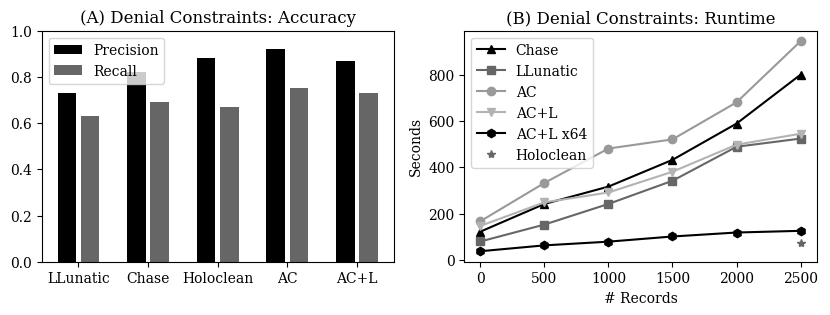
\includegraphics[width=\columnwidth]{exp/exp1.png}
    \caption{We compare \sys to alternative denial constraint systems on a dataset of flight arrival and departure times scraped from a variety of different sources. AC denotes \sys without any learned pruning and AC+L denotes \sys with pruning.
    \sys matches the accuracy of these systems and can be parallelized to match the runtime of these systems as well. Learning actually allows \sys to scale sub-linearly, i.e., as it sees more data it learns more precise pruning rules.\label{exp1a}}
\end{figure}

\subsection{Comparisons with Specialized Cleaning}
This subsection compares \sys to specialized cleaning approaches.  We illustrate that \sys can achieve comparable or higher accuracy, and the trade-offs in its runtime performance as compared to the baselines.

\subsubsection{Denial Constraints}
Denial constraints express a wide range of integrity constraints and form the basis of many data cleaning systems~\cite{llunatic,chase,holoclean}.  Although \sys may not fully enforce integrity constraints, we can compose a quality function can quantifies the number of constraint violations and find transformation that reduce the number of violations.    We use the Flight dataset for these experiments.

% Several data cleaning systems use Denial Constraints for constraint specification.  While \sys does not enforce integrity constraints, we can create a data quality objective function that quantifies the number of unsatisfied constraints.  This will search over a set of transformations that maximally satisfy these constraints.

\stitle{Baselines} We run against (1) Llunatic, a denial constraint-based cleaning system~\cite{DBLP:conf/sigmod/DallachiesaEEEIOT13} implemented in C++ on top of PostgreSQL, and (2) a restricted chase algorithm~\cite{benedikt2017benchmarking} implemented in Python. We compare against the chase because a large portion of denial constraints are functional dependencies~\cite{}, and can be resolved using fixed-point iteration.  We report numbers from the recent Holoclean publication~\cite{rekatsinas2017holoclean} that used the same datasets and constraints, but did not run the experiment ourselves.

\stitle{Results: } Figure \ref{exp1a}a shows the precision and recall of each approaches based on known ground truth. \sys matches or beats the accuracy of the baselines, however its runtime (AC) without any learning scales poorly compared to alternatives (\Cref{exp1b}b).  Using learning (AC+L) shows performance on par with LLunatic, and parallelization on 64 threads is comparable to Holoclean's reported runtime. The results suggest that learning exhibits sublinear scaling due to \sys learning more effective pruning rules as it sees more data.  These performance gains are at the expense of slightly reduced accuracy. 

We also evaluated \sys (single threaded, without learning) on the FEC, Malasakit, and Physician datasets, and summarize the results below:
\begin{table}[ht]
\footnotesize
\small
\centering
\begin{tabular}{|l|r|r|r|r|r|r|r|}
\hline
 & \#rows & \#cols & Precision & Recall & Runtime \\
\hline
\hline
FEC	&6M&18&0.94&	0.68&	5hrs\\
\hline
Malasakit &1493& 15& 1.0 & 0.85& 0.39hrs\\
\hline
Physican	&37k&10&1.0&0.84& 3.2hrs\\
\hline
\end{tabular}
\end{table}

\begin{figure}
    \centering
    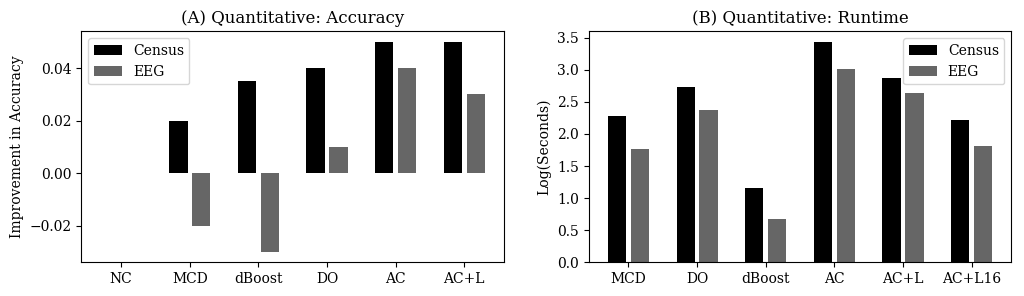
\includegraphics[width=\columnwidth]{exp/exp2.png}
    \caption{\ewu{REMOVE NO CLEAN FROM PLOT} We evaluate \sys on a quantitative data cleaning task by cleaning a dataset prior to training a random forest classifier model. The system is allowed to clip outliers or set them to a default value. (A) reports the resulting classifier accuracy improvements as compared to outlier detection algorithms (MCD,dBoost) and \sys with only a single transform template (DO).  (B) reports the runtimes.  \label{exp2a}}
\end{figure}

\subsubsection{Quantitative Data Cleaning}
This experiment performs numerical cleaning on machine learning data.  In these applications, prediction labels and test records are typically clean and available (e.g., results of a sales lead), whereas the training features are often integrated from disparate sources and exhibit considerable noise (e.g., outliers).  Our quality function is simply defined as the model's accuracy on a training hold-out set, and we report the test accuracy on a separate test set.

We trained a binary classification random forest model using \texttt{sklearn} on the Census and EEG datasets.  We used standard featurizers (hot-one encoding for categorical data, bag-of-words for string data, numerical data as is) similar to~\cite{gokhale2014corleone}. 
\ewu{We split the dataset into 20\% test and 80\% training, and further split training into 20/80 into hold-out and training.  We run the search over the training data, and evaluate the quality function using the hold-out.  Final numbers are reported using the test data.  }


% The quality function for \sys is 0 for each record that is incorrectly predicted by the model, 1 for each record that is correctly predicted by the model.


% In many machine learning settings, cleanly labeled test data is often available (e.g., the results of following a sales lead). 
% Labels often represent directly observed phenomena making them relatively clean, while features are often weaker signals integrated from multiple disparate sources and subject to error and frequent change.
% This allows us to define a quality function in terms of the model's predictive accuracy--the data cleaning being a means to improving that predictive accuracy.

We defined the following three data transformation templates that sets numerical attribute values in $R$ if they satsify a predicate:

{\small
\begin{itemize}[leftmargin=*, topsep=0mm, itemsep=0mm]
  \item \stitle{\textsf{clip\_gt(attr, thresh)}} $R.attr = thresh$ if $R.attr>thresh$
  \item \stitle{\textsf{clip\_lt(attr, thresh)}} $R.attr = thresh$ if $R.attr<thresh$
  \item \stitle{\textsf{default(attr, badval)}} $R.attr$ set to mean val if $R.attr=badval$
\end{itemize}
}

\stitle{Baselines} We compare with 4 baselines: {\it No Cleaning (NC)}, {\it Minimum Covariance Determinant (MCD)} is a robust outlier detection algorithm used in~\cite{bailis2016macrobase} and sets all detected outliers to the mean value, {\it dBoost} uses a fast partitioned histogram technique to detect outliers~\cite{mariet2016outlier}, and {\it Default Only (DO)} runs \sys with only the \textsf{default()} transformation.  

\stitle{Results} The classifer achieves 82\% and 79\% accuracy on the uncleaned census and EEG data, respectively.  Most outliers in the census data are far from the mean, so MCD and dBoost can effectively find.  Further, setting census outliers to the mean is sensible. However, the same fix is not appropriate for the EEG data; it is better to clip the outlier values, thus MCD, dBoost, and DO have negligible or negative impact on accuracy.  When we realized this from running DO, it was straightforward to add the clipping transformations to the language, and with no other changes, re-run \sys with drastically improved EEG accuracies.  

Vanilla \sys (AC) is nearly $10\times$ slower than MCD, but the adding learning and 16-thread parallelization  matches MCD's runtimes.  dBoost is specialized for fast outlier detection and \sys is unlikely to match its runtime.  


\begin{figure}
    \centering
    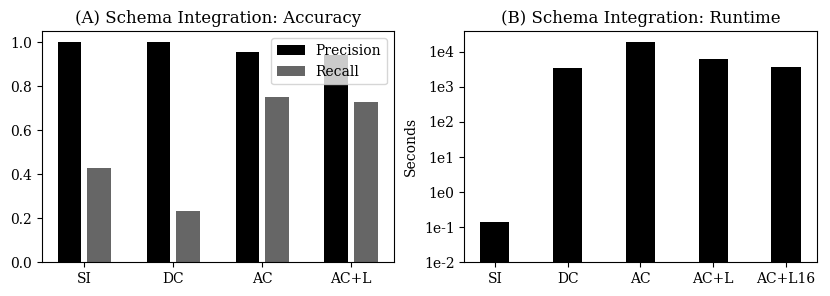
\includegraphics[width=\columnwidth]{exp/exp3.png}
    \caption{The stock dataset requires both schema integration (it contains data from 55 different sources) and functional dependency fixes.  Performing schema integration (SI) or data cleaning by enforcing functional dependencies (DC) in isolation results in poor accuracy.  \sys supports both types of errors, produces higher recall fixes, and can run comparably as fast as DC.  \label{exp3a}}
\end{figure}

\subsubsection{Schema Integration}
We now evaluate cleaning on the stock dataset~\cite{data-flights} from 55 different sources that contains a mixture of schema integration and functional dependency errors.

\vspace{0.5em}\noindent\textbf{Baselines: } We compare approaches for each error type in isolation.  Schema Integration  (SI) matches attributes based on attribute name string similarity, and Data Cleaning (DC) assumes schemas are consistent and enforces functions dependencies using a restricted chase~\cite{benedikt2017benchmarking}.

\vspace{0.5em}\noindent\textbf{Results: } The specialized cleaning approaches exhibit high precision but low recall, as they miss records with multiple errors (\Cref{exp3a}).  \sys can mix both tasks in the quality function and has comparable precision with much higher recall.  SI is significantly faster since it only reads schema metadata, however \sys with learning and 16 threads is competitive with DC.  
\begin{figure*}[ht]
\centering
 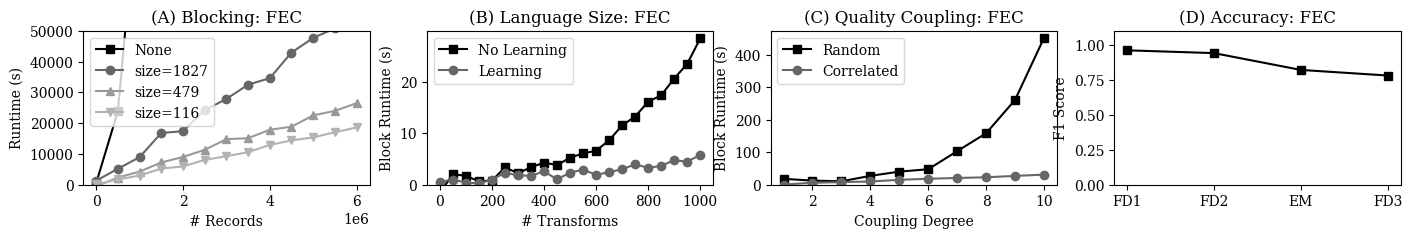
\includegraphics[width=\textwidth]{exp/exp4.png}
 \caption{(A) illustrates how the performance of \sys is affected block size, larger blocks require a longer search time, (B) shows how the search time scales as a function of the support of the transformation language, and learning can significantly reduce this time, (C) quality functions that have unpredictable couplings between multiple records together are harder to optimize, (D) \sys can handle compositions of multiple error types.
 \label{fig:microbenchmarks}}
\end{figure*}

\subsection{\sys In Depth}
This subsection studies the key parameters that affect \sys's accuracy and runtime, the robustness of its cleaning programs, and its algorithmic properties.

\subsubsection{Key Variables}
First, we evaluate which parameters affect the difficulty of the search problem. We start with the FEC dataset described in the previous experiments. 

\vspace{0.5em}\noindent \textbf{Blocking: } Partitioning the dataset into smaller pieces effectively reduces the search horizon. For example, consider a dataset of 1000 records where each record requires an independent transformation. Rather than solving a search problem of depth 1000, we can solve 1000 search problems of depth 1.
The maximum granularity of blocks depends on the nature of the transformations and quality functions.
Currently, these blocks are set by the user in the form of predicates that partition the dataset.
Figure \ref{fig:microbenchmarks}a illustrates how the performance of \sys is affected block size. We partition the FEC dataset on three different attributes each with a different blocksize. The smaller the blocks the better the algorithm scales with the data. Without blocking, on this dataset, the search is very impractical.

\vspace{0.5em}\noindent \textbf{Language: } The next experiment (Figure \ref{fig:microbenchmarks}b) shows how the search time within a block scales as a function of the support of the transformation language. The more transformations there are, the higher the branching factor of the search problem. Without any optimizations, the search time is exponential in the language. But, once a pruning model is learned this time is significantly reduced.

\vspace{0.5em}\noindent \textbf{Quality Function Structure: } The nature of the quality function also affects the search time. Quality functions that couple multiple records together are harder to optimize (Figure \ref{fig:microbenchmarks}c).
Consider a function that requires that two different records must have the same attribute values.
More transformations have to be achieved in a particular sequence before an improvement in quality is observed. 
We selected between 1-10 records at random in each block and created a quality function that coupled these records together.
As the degree of coupling increases, the search time grows quite drastically.
We repeated the same experiment where now coupling is correlated with the data, i.e., we sort one of the attributes and couple ``nearby'' records.
\sys performs significantly better on this version of the task.
This is due to the learned pruning in \sys.
Sorting the attributes introduces a systematic correlation in the quality function.
\sys quickly learns a model which learns this correlation and uses that to prune the search space.

To illustrate how the structure of the quality function affects accuracy, we incrementally make the FEC data cleaning problem more difficult.
We first start with a single FD, then add another, then add rules to match entities, and then another FD.
The quality function used is a sum of the quality functions for each of the constraints.
As the quality function considers more and more constraints, it becomes harder to optimize.

 \begin{figure*}[ht]
\centering
 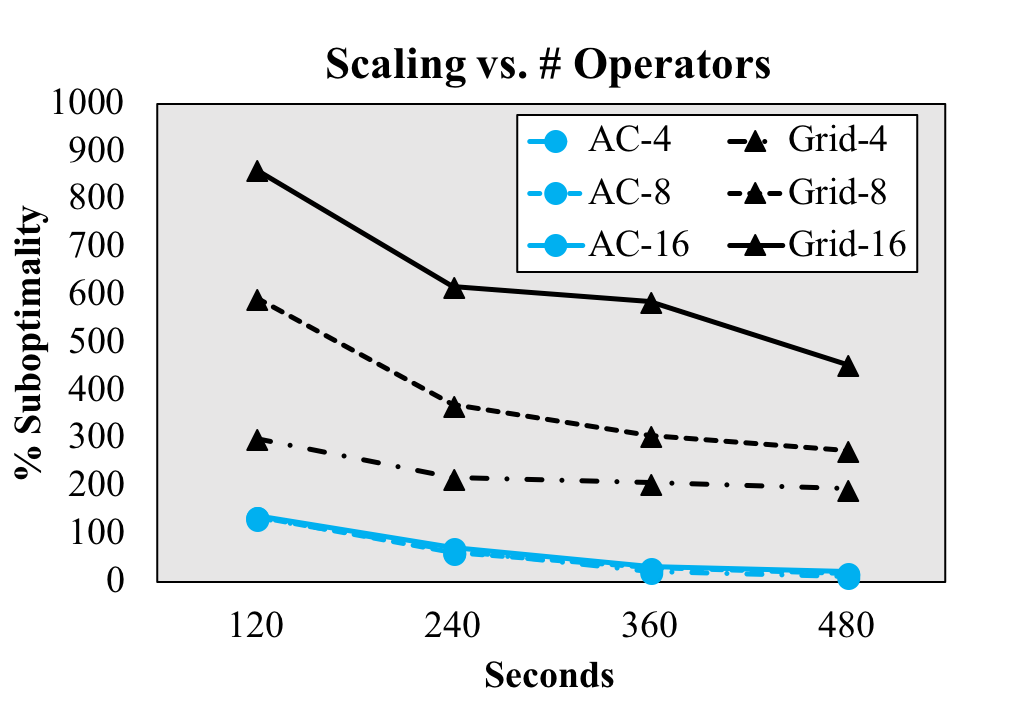
\includegraphics[width=\textwidth]{exp/exp5.png}
 \caption{ (A) We inject noise into the quality function to simulate a ``mis-specified'' objective and plot the F1 accuracy of \sys for different settings of the edit penalty, (B-C) overly specific rules may not apply to future data, and overly general rules, might introduce unwanted side-effects. \ewu{Change titles to TRaining and Test Accuracy}
 \label{fig:sensitivity}}
\end{figure*}

\subsubsection{Cleaning Generalization and Sensitivity}
An important characteristic of generating cleaning solutions as {\it programs} is that we can evaluate the program's robustness in terms of machine learning concepts such as overfitting and generalization.    To this end, we examine two concepts in the context of data cleaning: regularizaton and overfitting.  We also find that \sys's high level interface is helpful for iteratively tuning the cleaning process.

\stitle{Regularization}  Misspecified quality functions can cause \sys to output poorly performing cleaning programs.  We simulate this by adding random noise to the output of the quality function. \Cref{fig:sensitivity}A plots the F1-score of \sys on the FEC experiment while varying the amount of noise.  As expected, the output program's F1-score rapidly degrades as the noise increases.  

Machine learning uses regularizing penalty terms to prevent overfitting.  We can similarly add a penalty to the quality function to prevent too many edits.  Each line line shows the edit cost penalty and shows that although the F1 is lower when there is no noise, \sys is more robust to larger amounts of noise. 

\stitle{Overfitting} In machine learning, over-parameterized models may be susceptible to overfitting.  A similar property is possible if the language $\Sigma$ is overly expressive.  We use a transformation template that finds records matching a parameterized predicate and sets an attribute to another value in its instance domain.   We then vary the language expressiveness by increasing number of attributes in the predicate between 1 and 3.  Finally, we run \sys on a training sample of the dataset (x-axis), and report F1 accuracy on the training and a separate test sample (\Cref{fig:sensitivity}B-C).  Note that overfitting occurs when the training accuracy is significantly higher than test accuracy.

Indeed we find an interesting trade-off.  The 1 attribute predicate performed worst on the training sample but outperformed the alternatives on the test sample.  The 2 attribute predicate was more expressive and overfit to the training data.  Finally, the 3 attribute predicate is overly expressive and computationally difficult to search.  Thus, it did not sufficiently explore the search space to reliably identify high quality cleaning programs. 

\stitle{Discussion} We have shown that data cleaning can overfit, and believe this is a potential issue in {\it any} cleaning procedure. These results highlight the importance of domain experts to judge and constrain the cleaning problem in ways that will likely generalize to future data. Further, it shows the value of a high-level interface that experts can use to express these contraints by iteratively tuning the quality function and cleaning language. 

% and evaluate the training and test        Figure \ref{fig:sensitivity}B-C illustrates another interesting aspect of \sys, namely, a property akin to overfitting in machine learning.
% We parametrized the transformation language with single attribute, double attribute, and triple attribute predicates.
% Then, we applied \sys to sample of data.
% We measured the ``in-sample error'' Figure \ref{fig:sensitivity}C, which is the F1 score with records inside the sample, and the ``out-of-sample'' error which is the F1 score on unseen records.
% The more expressive two attribute predicates are most accurate on the in-sample metric, however, we not as accurate as the single attribute predicates on the out-of-sample metric.
% The three sample predicates were very computationally expensive to search so the results are less reliable.
% This result highlights an important point overly specific rules may not apply to future data, and overly general rules, might introduce unwanted side-effects.


\subsubsection{Algorithm Properties}
Finally, Figure \ref{fig:opt} illustrates the scaling properties of \sys. We run all of our experiments on a cluster of 4 mx.large EC2 instances. We compare three baseline implementations: (No opt.) a vanilla best-first search, (Cache) best-first search + materialization, (Cache+Comm) best-first search and reducing the communication with the algorithm described in the paper. 
Figure \ref{fig:opt}A shows how the run time on the FEC dataset varies as a function of the number of worker threads on the cluster.
With no optimizations and single threaded, the runtime is 4432 seconds.
If we use the materialization strategy described in the paper, we can reduce this runtime by a factor of 10 (432 seconds) even on a single thread.
As we scale out, we can further reduce this runtime.
We see that the Cache+Comm strategy scales better (67 seconds for 64 workers) than the naive Cache only strategy (137 seconds for 64 workers).
Interestingly enough, in relative terms, the vanilla best-first search strategy scales the best.
This is because with no materialization the only communication is the description of which transformations to expand.
However, it is slower by a factor of 10 in absolute numbers.

Figure \ref{fig:opt}B illustrates the effect of learning a search heuristic. As more blocks are cleaned, the system trains a classifier to prune implausible transformations in the future.
This means that the search time spent on each block is greatly reduced (75\%). 
Figure \ref{fig:opt}C shows that the best-first search is really the most practical algorithm in this setting, running order of magnitudes faster than a naive BFS or DFS.

 \begin{figure*}[ht]
\centering
 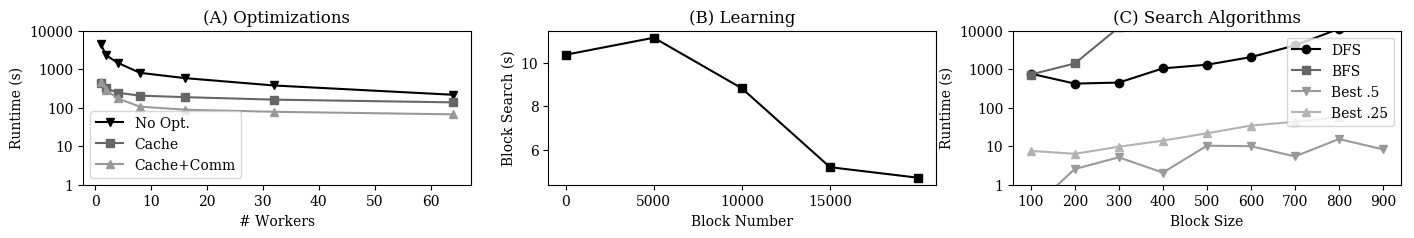
\includegraphics[width=\textwidth]{exp/exp6.png}
 \caption{(A) We compare three baseline implementations for scalability: (No opt.) a vanilla best-first search, (Cache) best-first search + materialization, (Cache+Comm) best-first search and reducing the communication with the algorithm described in the paper. (B) illustrates the effect of learning a search heuristic. (C) best-first search is much more effective than a BFS or DFS search.
 \label{fig:opt}}
\end{figure*}

